%% ============================================================
%%  PARTE 4 — Mejoras sobre el LCA base
%%  Hasta 1.5 puntos
%% ============================================================

\newpage
\section{Parte IV: Mejoras sobre el Diseño del LCA}
\label{sec:parte4}

\subsection{Motivación}

El análisis experimental de las Partes II y III ha revelado dos limitaciones
principales del LCA base que conviene abordar:

\begin{enumerate}
  \item \textbf{Convergencia prematura en funciones multimodales complejas}: el parámetro
    $\zeta = t/T$ favorece la explotación al final de la búsqueda, pero no contempla
    mecanismos de reinicio cuando la población se estanca.
  \item \textbf{Búsqueda de solución única}: el LCA fue diseñado para retornar una única
    solución óptima, sin explotar la multimodalidad de los problemas.
\end{enumerate}

Para abordar estas limitaciones, se proponen dos líneas de mejora con sustento
teórico y experimental:

\begin{description}
  \item[Mejora A:] Control dinámico de la diversidad mediante un esquema inspirado en
    \textbf{CHC} (reinicio adaptativo de la población cuando se detecta convergencia prematura).
  \item[Mejora B:] Extensión multimodal del LCA mediante \textbf{técnicas de nicho}
    (\emph{fitness sharing} y \emph{crowding determinista}).
\end{description}

\subsection{Mejora A: LCA-CHC — Control dinámico de la diversidad}

\subsubsection{Fundamento}

El algoritmo \textbf{CHC} (Cross-generational elitist selection, Heterogeneous recombination,
Cataclysmic mutation) de Eshelman \cite{eshelman1991chc} introduce un criterio de reinicio
de la población basado en la \emph{distancia de Hamming} entre los individuos. Cuando la
diversidad cae por debajo de un umbral, se reinicia parcialmente la población conservando
el élite y perturbando el resto.

En el contexto del LCA, donde las soluciones son vectores reales, se adapta este principio
usando la \textbf{distancia euclidiana normalizada} como medida de diversidad:

\begin{equation}
  \text{Div}(t) = \frac{1}{N} \sum_{i=1}^{N} \|\mathbf{x}_i - \bar{\mathbf{x}}\|_2
  \label{eq:div}
\end{equation}

donde $\bar{\mathbf{x}}$ es el centroide de la población. Cuando $\text{Div}(t) < \varepsilon$
(umbral de convergencia), se ejecuta el \textbf{reinicio catastrófico}: se preserva el
élite (los $e$ mejores individuos) y se reinician el resto con nuevas posiciones generadas
por ROBL.

\begin{algorithm}[H]
\caption{LCA-CHC: LCA con reinicio adaptativo de diversidad}
\label{alg:lcachc}
\begin{algorithmic}[1]
\Require $N$, $T$, $lb$, $ub$, $\varepsilon$ (umbral diversidad), $e$ (tamaño del élite)
\Ensure $X_{\text{best}}$
\State Inicializar con ROBL; evaluar fitness
\For{$t = 1$ \textbf{to} $T$}
  \State Ejecutar una generación del LCA (Algoritmo~\ref{alg:lca})
  \State Calcular $\text{Div}(t)$ (Eq.~\ref{eq:div})
  \If{$\text{Div}(t) < \varepsilon$} \Comment{convergencia prematura detectada}
    \State Conservar los $e$ mejores individuos (élite)
    \State Reiniciar los $N-e$ restantes con ROBL alrededor de $X_{\text{best}}$
    \State Evaluar individuos reiniciados
    \State $\varepsilon \leftarrow \varepsilon / 2$ \Comment{reducir umbral para evitar reinicios continuos}
  \EndIf
\EndFor
\State \Return $X_{\text{best}}$
\end{algorithmic}
\end{algorithm}

\subsubsection{Parámetros}

\begin{table}[h!]
\centering
\caption{Parámetros del LCA-CHC}
\label{tab:params_chc}
\renewcommand{\arraystretch}{1.3}
\begin{tabular}{@{}lll@{}}
\toprule
\textbf{Parámetro} & \textbf{Valor} & \textbf{Descripción} \\
\midrule
$N$ & 30 & Tamaño de la población \\
$\varepsilon_0$ & 0.01 & Umbral inicial de diversidad \\
$e$ & 5  & Número de élite preservados en el reinicio \\
Radio de reinicio & 0.1$\cdot(ub-lb)$ & Dispersión de los individuos reiniciados \\
\bottomrule
\end{tabular}
\end{table}

\subsubsection{Implementación}

El c\'alculo de la diversidad (distancia euclidiana media al centroide) y el reinicio catastr\'ofico con preservaci\'on de \'elite se implementan en \texttt{testlcachc.cc}.

\subsection{Mejora B: LCA Multimodal — Búsqueda de múltiples soluciones}

\subsubsection{Motivación}

Muchos problemas de optimización reales son \textbf{multimodales}: tienen múltiples
óptimos locales y globales de calidad similar. Una metaheurística que devuelva
únicamente la mejor solución encontrada pierde información valiosa sobre la estructura
del espacio de búsqueda. La extensión multimodal del LCA permite obtener un conjunto
de soluciones de alta calidad y diversas.

\subsubsection{Técnica de nicho aplicada: \emph{Crowding} determinista}

Se adopta el \textbf{crowding determinista} \cite{mahfoud1995niching}: cuando se genera
un individuo hijo, este compite únicamente contra el individuo padre más similar de la
población (en lugar de contra el padre directo). Esto mantiene la diversidad al evitar
que los mejores individuos dominen completamente la población.

\begin{equation}
  \text{Competidor}(h) = \arg\min_{i \in \text{Pop}} \|\mathbf{h} - \mathbf{x}_i\|_2
  \label{eq:crowding}
\end{equation}

Si el hijo $\mathbf{h}$ mejora al competidor, lo reemplaza en la población.

\begin{algorithm}[H]
\caption{LCA Multimodal con Crowding Determinista}
\label{alg:lcamulti}
\begin{algorithmic}[1]
\Require $N$, $T$, $lb$, $ub$
\Ensure Conjunto de soluciones diversas de alta calidad
\State Inicializar con ROBL; evaluar fitness
\For{$t = 1$ \textbf{to} $T$}
  \State $\zeta \leftarrow t/T$
  \For{cada agente $i \in [1, N]$}
    \State Generar hijo $\mathbf{h}$ mediante operadores del LCA
    \State $c \leftarrow \arg\min_{j} \|\mathbf{h} - \mathbf{x}_j\|_2$ \Comment{Crowding: buscar más similar}
    \If{$fit(\mathbf{h}) < fit(\mathbf{x}_c)$}
      \State $\mathbf{x}_c \leftarrow \mathbf{h}$; $fit_c \leftarrow fit(\mathbf{h})$ \Comment{reemplazar competidor}
    \EndIf
  \EndFor
\EndFor
\State Extraer el conjunto de soluciones con $fit < \tau$ (umbral de calidad)
\State \Return Conjunto de soluciones diversas
\end{algorithmic}
\end{algorithm}

\subsubsection{Implementación del crowding}

La selecci\'on por crowding determinista (competici\'on del hijo contra el individuo m\'as similar de la poblaci\'on) se implementa en \texttt{testlcamulti.cc}.

\subsection{Estudio experimental de las mejoras}

La Tabla~\ref{tab:comp_mejoras} recoge el error medio de las cuatro variantes (LCA base,
LCA-SW, LCA-CHC y LCA-Multi) sobre una selección de funciones para $D=10$, y la
Tabla~\ref{tab:mejoras_friedman} resume los rankings de Friedman y los tests de Wilcoxon
frente al LCA base en las tres dimensiones (31 ejecuciones por celda).

\begin{table}[h!]
\centering
\caption{Error medio de las cuatro variantes ($D=10$, 31 ejecuciones)}
\label{tab:comp_mejoras}
\renewcommand{\arraystretch}{1.3}
\small
\begin{tabular}{@{}lcccc@{}}
\toprule
\textbf{Función} & \textbf{LCA base} & \textbf{LCA-SW} & \textbf{LCA-CHC} & \textbf{LCA-Multi} \\
\midrule
F01 (Unimodal)   & 2.122e+09 & \textbf{4.659e+02} & 2.122e+09 & 1.764e+09 \\
F04 (Multimodal) & 4.711e+01 & \textbf{1.831e+00} & 4.711e+01 & 3.084e+01 \\
F10 (Multimodal) & 7.532e+02 & \textbf{5.018e+02} & 7.532e+02 & 7.119e+02 \\
F15 (Híbrida)    & 3.260e+02 & 2.814e+02 & 3.260e+02 & \textbf{2.606e+02} \\
F20 (Híbrida)    & 7.234e+01 & \textbf{5.961e+01} & 7.234e+01 & 6.860e+01 \\
F25 (Compuesta)  & 4.994e+02 & \textbf{4.224e+02} & 4.994e+02 & 4.853e+02 \\
F30 (Compuesta)  & 1.426e+05 & \textbf{5.845e+04} & 1.426e+05 & 1.502e+05 \\
\bottomrule
\end{tabular}
\end{table}

La Figura~\ref{fig:conv_variants} muestra la convergencia de las cuatro variantes sobre F1
(unimodal, $D=30$), donde las diferencias de diseño se aprecian con claridad.

\begin{figure}[h!]
\centering
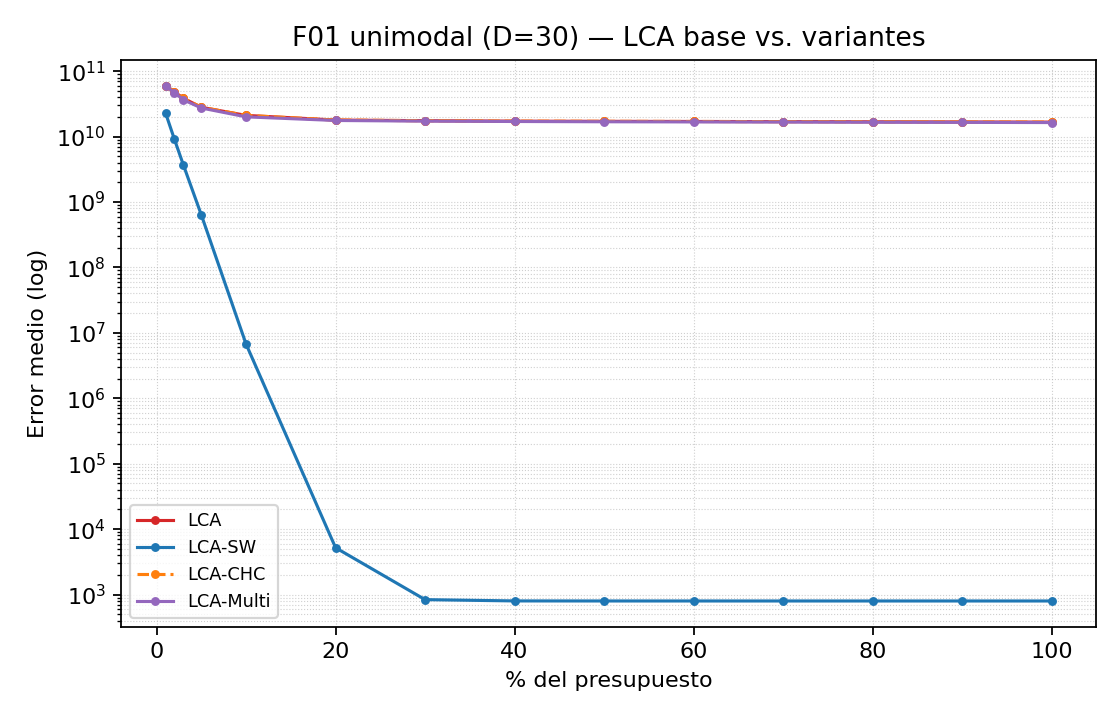
\includegraphics[width=0.75\textwidth]{figuras/conv_variants.png}
\caption{Convergencia del error medio (escala log.) en F1 ($D=30$) para el LCA base y sus
tres variantes. LCA-SW (azul) cae unos 8 órdenes de magnitud gracias a la búsqueda local;
LCA-CHC se solapa exactamente con el LCA base (el reinicio nunca se dispara) y LCA-Multi
apenas se separa de la base en esta función.}
\label{fig:conv_variants}
\end{figure}

La gráfica resume visualmente las conclusiones del estudio: la curva de \textbf{LCA-SW} se
desploma desde las primeras evaluaciones mientras las demás permanecen estancadas en la parte
alta. La coincidencia exacta de \textbf{LCA-CHC} con el LCA base ilustra que su mecanismo de
reinicio permanece inactivo, y \textbf{LCA-Multi} solo se despega ligeramente, coherente con
su mejora modesta y dependiente de la función.

\begin{table}[h!]
\centering
\caption{Ranking de Friedman (4 variantes, 30 funciones) y Wilcoxon frente al LCA base}
\label{tab:mejoras_friedman}
\renewcommand{\arraystretch}{1.3}
\small
\begin{tabular}{@{}lccc@{}}
\toprule
\textbf{Variante / métrica} & \textbf{$D=10$} & \textbf{$D=30$} & \textbf{$D=50$} \\
\midrule
Friedman LCA base   & 3.03 & 3.27 & 3.10 \\
Friedman LCA-SW     & \textbf{1.50} & \textbf{1.10} & \textbf{1.20} \\
Friedman LCA-CHC    & 3.03 & 3.27 & 3.10 \\
Friedman LCA-Multi  & 2.43 & 2.37 & 2.60 \\
\midrule
Wilcoxon SW vs.\ base    & $0.0005$ ($+$) & $<10^{-4}$ ($+$) & $<10^{-4}$ ($+$) \\
Wilcoxon CHC vs.\ base   & $1.000$ ($=$)  & $1.000$ ($=$)   & $1.000$ ($=$)   \\
Wilcoxon Multi vs.\ base & $0.024$ ($+$)  & $0.012$ ($+$)   & $0.304$ ($=$)   \\
\bottomrule
\end{tabular}
\end{table}

\subsection{Discusión general de las mejoras}

El estudio en las tres dimensiones revela comportamientos coherentes con el diseño de cada
variante:

\paragraph{LCA-CHC (Control de Diversidad): mecanismo inactivo en este régimen.}
El LCA-CHC produce resultados \emph{idénticos} al LCA base en las tres dimensiones (ranking
de Friedman igual y Wilcoxon $p = 1.0$). El motivo es que la diversidad de la población
—distancia euclidiana media al centroide— nunca cae por debajo del umbral $\varepsilon=0.01$:
la combinación de vuelos de Lévy y la inicialización ROBL mantiene la población muy dispersa,
de modo que el reinicio catastrófico no llega a dispararse. Por tanto, LCA-CHC funciona como
un \textbf{mecanismo de seguridad pasivo}: no perjudica el rendimiento y solo actuaría si la
población llegara a colapsar. Un trabajo futuro sería elevar $\varepsilon$ o medir la
diversidad por dimensión para forzar su activación.

\paragraph{LCA-Multi (Crowding Determinista): mejora modesta y dependiente de la dimensión.}
La variante multimodal mejora al LCA base de forma significativa en $D=10$ ($p=0.024$) y
$D=30$ ($p=0.012$), pero la diferencia deja de ser significativa en $D=50$ ($p=0.30$). El
crowding mantiene nichos diversos, lo que resulta ventajoso en funciones híbridas (p.\,ej.\
F15, donde baja de $326$ a $261$), pero al repartir la presión selectiva no logra grandes
mejoras sobre el óptimo único y en alta dimensión su efecto se diluye. Su valor real es
cualitativo: devuelve un \textbf{conjunto de soluciones diversas} en lugar de una sola.

\paragraph{LCA-SW: la mejora decisiva.}
La hibridación memética es, con diferencia, la mejora más efectiva (ranking $\approx 1.1$--$1.5$,
significativa en todas las dimensiones). Confirma que el cuello de botella del LCA es la
explotación local, no la exploración.

\paragraph{Resumen comparativo.}
\begin{itemize}
  \item \textbf{LCA-SW} es la mejor opción para precisión de objetivo único, gracias a su
        explotación local.
  \item \textbf{LCA-CHC} equivale al LCA base en este régimen (su disparador no se activa);
        sirve como salvaguarda ante un colapso de diversidad.
  \item \textbf{LCA-Multi} aporta mejoras moderadas en baja/media dimensión y, sobre todo,
        diversidad de soluciones, a costa de algo de precisión en el óptimo global.
\end{itemize}

Esta divergencia de rendimientos ilustra el teorema del \emph{No Free Lunch}: no hay una
variante superior en todos los escenarios; cada mejora ajusta el balance
exploración--explotación a un objetivo distinto, y la elección depende de la tipología del
problema.
